\documentclass[graybox]{svmult}

% choose options for [] as required from the list
% in the Reference Guide

\usepackage{mathptmx}       % selects Times Roman as basic font
\usepackage{helvet}         % selects Helvetica as sans-serif font
\usepackage{courier}        % selects Courier as typewriter font
\usepackage{type1cm}        % activate if the above 3 fonts are
                            % not available on your system
\usepackage{makeidx}         % allows index generation
\usepackage{multicol}        % used for the two-column index
\usepackage[bottom]{footmisc}% places footnotes at page bottom

%% personal packages
\usepackage{amsmath,amssymb}
\usepackage{xcolor}
\usepackage{natbib}
\usepackage{enumerate}
\usepackage{macros}

\usepackage{centernot}
\usepackage[textwidth=8em,textsize=small]{todonotes}
\usepackage[ruled,vlined]{algorithm2e}
\usepackage{graphicx}

\usepackage{tikz}
\usetikzlibrary{calc,shapes,backgrounds,arrows,automata,shadows,positioning}
\usepackage{multirow}
\definecolor{mblue}{RGB}{94,135,173}
\colorlet{mred}{red!80!black}

\graphicspath{{./figures/}}

\begin{document}

\title*{A multiattribute Gaussian graphical model for inferring
  multiscale regulatory networks: an application in breast cancer}
\titlerunning{Multiattribute GGM for multiscale regulatory networks}
\author{Julien Chiquet, Guillem Rigaill and Martina Sundqvist \\
  \textit{AgroParisTech, INRA, Universit\'e Paris-Saclay}}
\authorrunning{Chiquet \textit{et al.}}
\institute{%
  Julien Chiquet \at MIA Paris, AgroParisTech/INRA, 16 rue Claude Bernard, 75231 Paris CEDEX 05, France \newline \email{julien.chiquet@inra.fr} \and
  Martina Sundqvist \at MIA Paris, AgroParisTech/INRA, 16 rue Claude Bernard, 75231 Paris CEDEX 05, France \newline \email{martina.sundqvist@agroparistech.fr} \and
  Guillem Rigaill \at IPS2, B\^atiment 630, Rue de Noetzlin, Plateau du Moulon, 91405 Orsay, France  \newline \email{guillem.rigaill@inra.fr}}



\maketitle

\abstract{. This chapter addresses the problem of reconstructing
  regulatory networks in molecular biology by integrating multiple
  sources of data. We consider data sets measured from diverse
  technologies all related to the same set of variables and
  individuals. This situation is becoming more and more common in
  molecular biology, for instance when both proteomic and
  transcriptomic data related to the same set of ``gene'' are
  available on a given cohort of patients.\newline \indent To infer a
  consensus network that integrates both proteomic and transcriptomic
  data, we introduce a multivariate extension of Gaussian graphical
  models (GGM), which we refer to as \textit{multiattribute}
  GGM. Indeed, the GGM framework offers a good proxy for modeling
  direct links between biological entities. We perform the inference
  of our multivariate GGM with a neighborhood selection procedure that
  operates at a multiscale level. This procedure employs a group-Lasso
  penalty in order to select interactions which operate both at the
  proteomic and the transcriptomic level between two genes. We end up
  with a \textit{consensus} network embedding information shared at
  multiple scales of the cell. We illustrate this method on two breast
  cancer data sets.}

\keywords{Multiscale Regulatory Network $\cdot$ Gaussian Graphical
  Model $\cdot$ Group-Lasso $\cdot$ Proteomic Data $\cdot$ Multi-Omic
  Data}

\section{Introduction}

\paragraph*{Gaussian Graphical Models (GGMs): a canonical framework
  for network inference modeling.} Gaussian Graphical Models (GGMs)
\citep{1996_Book_Lauritzen,whittaker1990graphical} are a very
convenient tool for describing the patterns at play in complex data
sets.  Indeed, through the notion of partial correlation, they provide
a well-studied framework for spotting direct relationships between
variables, and thus reveal the latent structure in a way that can be
easily interpreted. Application areas are very broad and include for
instance gene regulatory network inference in biology (using gene
expression data) as well as spectroscopy, climate studies, functional
magnetic resonance imaging, etc.  Estimation of GGMs in a sparse,
high-dimensional setting has thus received much attention in the last
decade, especially in the case of a single homogeneous data set
\citep{2006_AS_Meinshausen,2007_BS_Friedman,2008_JMLR_Banerjee,2010_JMLR_Yuan,2011_AS_Cai}.

However, this simple canonical setup is uncommon in real world data
sets, because of both the complexity of the mechanism at play in
biology and the multiplicity of the sources of data in omic. Hence,
the need for variants of sparse GGM more adapted to recent omic data
set is huge.

As a first example, the work developed in \cite{2009_EJS_Chiquet,
  2009_BI_Chiquet} addresses the introduction of a possible special
organization of the network itself to drive the reconstruction
process.  Indeed, while sparsity is necessary to solve the problem
when few observations are available, biasing the estimation of the
network towards a given topology can help us find the correct graph in
a more robust way, by preventing the algorithm from looking for
solutions in regions where the correct graph is less likely to
reside. As a second example, \cite{2011_SC_Chiquet} addresses the
problem of sample heterogeneity which typically occurs when several
assays are performed in different experimental conditions that
potentially affect the regulations, but are still merged together to
perform network inference as data is very scarce.  We remedy
heterogeneity among sample experiments by estimating multiple GGMs,
each of which matches different modalities of the same set of
variables, which correspond here to the different experimental
conditions. This idea, coupled with the integration of biological
knowledge, was further explored for application in cancer in
\cite{2014_inbook_jeanmougin}.

A deeper generalization of GGM comes by integrating multiple types of
data measured from diverse platforms, what is sometimes referred to as
\emph{horizontal} integration: not only does this means a better
treatment of the heterogeneity of the data, but it also makes the
network reconstruction more robust. The model presented in this
chapter gives an answer to this question by offering a solution to
reconstruct a sparse, multiattribute GGM, recoursing on both proteomic
and genomic data to infer a consensus network. Our main motivating
application is a better understanding of heterogeneity in breast
cancer, as detailed below.

\paragraph*{Proteomic and Transcriptomic data integration in cancer.} 
Protein deregulations, leading to abnormal activation of signaling
pathways, contribute to tumorigenesis
\citep{giancotti2014deregulation}. Knowing the level of activation of
the signaling pathways in any subgroup of tumors could therefore be a
key indication to understand the biological mechanisms involved in
tumorigenesis, and to identify some therapeutic targets.  % Protein
% expression levels are poorly predicted by RNA expression data
% \citep{akbani2014pan}. Moreover, proteins are also regulated by
% post-translational modifications, such as phosphorylation.  These
% post-translational modifications play essential roles in cell function
% by regulating the intracellular signaling pathways involved in diverse
% processes such as metabolism, transcription, differentiation,
% cytoskeleton rearrangement, apoptosis, intercellular communication and
% proliferation \citep{johnson2009regulation}.
%
%% 2) Not a lot of protein data (not many samples, not many proteins)
% The post-translational modifications which regulate the activity of
% proteins and therefore impact signaling pathway activity cannot be
% detected in the RNA level.
Therefore, the analysis of proteins is
essential.  However, measuring the expression of proteins is more
difficult to implement than the measure of transcriptome (RNA) or
genome (DNA).  Several technologies have been developed to measure the
proteome, but the number of samples and the number of proteins that
can be studied simultaneously is, up to now, limited.  A useful
technique for this task is the RPPA (Reverse Phase Protein
Arrays). It allows studying protein expression levels and the activity
status of a few hundred proteins by analyzing their phosphorylated
state, in several hundred of samples \citep{akbani2014realizing}.

%% 3) Study both RNA and proteins to ... get a better understanding of
%% the underlying biological mechanism involved in (breast) cancer(?)
To summarize, better understanding the proteome of tumors is essential
to further our knowledge of cancer cells but proteome data are still
small and rare.  Integration of proteomic and transcriptomic data is a
promising avenue to get the most of available proteomic datasets and
better understand the relatives roles of transcriptome and proteome.
To take into account the different levels of information, a solution
is to use multivariate GGM. Since it is probable that the proteomic
and transcriptomic heterogeneity in cancers is caused by some few
major underlying alterations, the hypothesis of proximity in between
networks seems reasonable.  Identifying commonalities between the
transcriptome and proteome networks should help the prediction of the
proteome using the transcriptome for which several large public cancer
data sets are available.

\paragraph*{Chapter Outline.} In the next section we give a 
quick overview of the literature of sparse GGM (models, basic
theoretical results, inference and software). This provides the reader
with the necessary material to approach the model at play in this
chapter, dedicated to multiattribute GGM, introduced in Section 3. In
Section 4 we perform some numerical studies: we demonstrate on
simulated data the superiority of our approach in several
scenarios. Then, two breast cancer data sets are used to illustrate
the reconstruction of multiscale regulatory networks.


\section{Background}
\label{sec:chap2:background}

This section provides an overview on the state-of-the-art
$\ell_1$-regularization methods for sparse GGM inference and their
most recent striking variants, insisting on their computational and
statistical properties.  This provides the reader with the necessary
material to approach the model at play in this chapter, dedicated to
multiattribute GGM.

\subsection{Basics on Gaussian graphical models}
\label{sec:chap2:background:ggm}

Let  $\mathcal{P}=\{1,\dots,p\}$  be  a  set  of  fixed  vertices  and
$X=(X_1,\dots,X_p)^\intercal$ a random vector describing a signal over
this set.   The vector  $X\in \Rset^p$ is  assumed to  be multivariate
Gaussian  with unknown  mean and  unknown covariance  matrix $\covm  =
(\Sigma_{ij})_{(i,j)\in\mathcal{P}^2}$.   No  loss  of  generality  is
involved    when   centering    $X$,   so    we   may    assume   that
$X\sim\mathcal{N}(\bzr_p,\covm)$. The covariance matrix $\covm$, equal
to  $\E(XX^\intercal)$  under the  assumption  that  $X$ is  centered,
belongs to the set  $\mathcal{S}_{p}^+$ of positive definite symmetric
matrices of size $p\times p$.

\paragraph*{Graph of  conditional dependencies.}  GGMs  endow Gaussian
random  vectors  with a  graphical  representation  $\graph$ of  their
\emph{conditional dependency structure}: two variables $i$ and $j$ are
linked  by an  undirected edge  $(i,j)$ if,  conditional on  all other
variables   indexed  by   $\mathcal{P}  \backslash   \{i,j\}$,  random
variables $X_i$ and  $X_j$ remain or become dependent.   Thanks to the
Gaussian assumption, conditional independence actually boils down to a
zero  conditional  covariance $\textrm{cov}(X_i,X_j  |  X_{\mathcal{P}
  \backslash \{i,j\}})$, or equivalently to a zero partial correlation
which  we  denote  by  $\rho_{ij}$,  the  latter  being  a  normalized
expression of the former.

Concretely, the  inference of a GGM  is based upon a  classical result
originally emphasized in  \cite{1972_Biometrics_Dempster} stating that
partial  correlations $\rho_{ij}$  are  actually  proportional to  the
corresponding entries  in the \emph{inverse} of  the covariance matrix
$\covm^{-1}  =   \invcov$,  also  known  as   the  \emph{concentration
  matrix}. More precisely, we have
\begin{equation}
  \label{eq:parcor2invcov}
  \rho_{ij}      =  -\invcov_{ij}      /
  \sqrt{\invcov_{ii} \invcov_{jj}}, \qquad \invcov_{ii}=
  \var(X_i|X_{\mathcal{P}\backslash i})^{-1};
\end{equation}
thus $\invcov$ directly describes the conditional dependency structure
of $X$. Indeed, after a simple rescaling, $\invcov$ can be interpreted
as the adjacency  matrix of an undirected  weighted graph representing
the partial  covariance (or  correlation) structure  between variables
$X_{1},\ldots,X_{p}$. Formally,  we denote by $\graph  = (\mathcal{P},
\mathcal{E})$ this graph, the edges of which are characterized by
\begin{displaymath}
  (i,j) \in \mathcal{E} \Leftrightarrow \invcov_{ij} \neq 0, \quad \forall
  (i,j) \in \mathcal{P}^2 \text{ such that } i\neq j.
\end{displaymath}
In words,  $\graph$ has  no self-loop and  contains all  edges $(i,j)$
such  that $\invcov_{ij}$  is nonzero.   Therefore recovering  nonzero
entries  of  $\invcov$  is  equivalent   to  inferring  the  graph  of
conditional dependencies  $\graph$, and the correct  identification of
nonzero entries is the main issue in this framework.

\paragraph*{Maximum Likelihood inference.}  GGMs  fall into the family
of  exponential  models  for  which   the  whole  range  of  classical
statistical tools applies.  As soon as  the sample size $n$ is greater
than  the number  $p$ of  variables,  the likelihood  admits a  unique
maximum  over  $\mathcal{S}_{p}^+$,   defining  a  maximum  likelihood
estimator  (MLE): suppose  we observe  a sample  $\set{X^1,\dots,X^n}$
composed of $n$  i.i.d.  copies of $X$, stored  row-wise once centered
in a matrix $\bX \in \Rset^{n\times  p}$ such that $(X^i)^\top$ is the
$i$th row  of $\bX$.   The empirical covariance  matrix is  denoted by
$\empcov   =  \mathbf{X}^\intercal   \mathbf{X}/n$.   Maximizing   the
likelihood is equivalent to
\begin{equation}
\label{eq:MLE_GGM}
\widehat{\invcov}^{\text{mle}} = \argmax_{\invcov  \in \mathcal{S}_p^+}\quad
\log \det(\invcov) - \trace(\invcov \empcov).
\end{equation}
When $n>p$, Problem \eqref{eq:MLE_GGM}  admits a unique solution equal
to  $\empcov$.   The  scaled  empirical  covariance  matrix  $\empcov$
follows  a  Wishart  distribution  while  its  inverse  $\empcov^{-1}$
follows an inverse Wishart distribution with computable parameters.

There are two  major limitations with the MLE  regarding the objective
of  graph  reconstruction  by  recovering the  pattern  of  zeroes  in
$\invcov$. First, it provides an  estimate of the saturated graph: all
variables  are connected  to each  other; second,  we need  $n$ to  be
larger than  $p$ to be  able to even  define this estimator,  which is
rarely the case in genomics. In  any case, the need for regularization
and feature selection is huge.  A  natural assumption is that the true
set of direct relationships between  the variables remains small, that
is, the  true underlying  graph is  sparse (say, of  the order  of $p$
rather than the  order of $p^2$).  Sparsity  makes estimation feasible
in  the  case where  $n<p$  since  we  can  concentrate on  sparse  or
shrinkage  estimators  with  fewer  degrees of  freedom  than  in  the
original problem.   Henceforth, the question of  selecting the correct
set  of edges  in  the graph  is  treated as  a  question of  variable
selection.

\paragraph*{High-dimensional inference of GGM.}  The different methods
for the inference of sparse GGMs in high-dimensional settings fall
into roughly three categories.  The first contains constraint-based
methods, performing statistical tests
\cite{2006_JMLR_Castelo,2007_SS_drton,2008_JSPI_drton,2011_BMC_Kiiveri,2006_SAGMB_Wille}.
However, they either suffer from the excessive computational burden
\cite{2006_JMLR_Castelo,2006_SAGMB_Wille} or strong assumptions
\cite{2007_SS_drton,2008_JSPI_drton} that correspond to regimes never
attained in real situations.  The second of these categories is
composed of Bayesian approaches, see for instance
\cite{2004_JMVA_Dobra,2005_SS_Dobra,rau2012reverse,schwaller2015tree}.
However, constructing priors on the set of concentration matrices is
not a trivial task and the use of MCMC procedures limits the range of
applications to moderate-sized networks.  The third category contains
regularized estimators, which add a penalty term to the likelihood in
order to reduce the complexity or degrees of freedom of the estimator
and more generally regularize the problem: throughout this chapter we
focus on $\ell_1$-regularized procedures, which are freed from any
test procedure -- and thus multiple testing issues -- since they
directly perform estimation and selection of the most significant
edges by zeroing entries in the estimator of $\invcov$.  The remainder
of this section is dedicated to a quick review of the state-of-the-art
methods of this kind.

\subsection{Sparse methods for GGM inference}
\label{sec:sparseGGM}

The idea underlying sparse methods for GGM is the same as for the
Lasso in linear regression \citep{1996_JRSS_Tibshirani}: it basically
uses $\ell_1$-regularization as a convex surrogate of the ideal but
computationally intensive $\ell_0$-regularized problem:
\begin{equation}
  \argmax_{\invcov  \in \mathcal{S}_p^+}\quad
  \log \det(\invcov) - \trace(\invcov \empcov) - \lambda\ 
  \|\invcov\|_{\ell_0}.
  \label{eq:ell0}
\end{equation}

Problem \eqref{eq:ell0} achieves a  trade-off between the maximization
of  the likelihood  and  the sparsity  of the  graph  within a  single
optimization problem.  The  penalty term can also be  interpreted as a
log prior  on the coefficients in  a Bayesian perspective. BIC  or AIC
criteria  are special  cases  of such  $\ell_0$ regularized  problems,
except  that the  maximization is  made  upon a  restricted subset  of
candidates  $\{\tilde{\Theta}_1,\dots,   \tilde{\Theta}_m\}$  and  the
choice of  $\lambda$ is fixed ($\log(n)$  for BIC and $1/2$  for AIC).
Actually solving \eqref{eq:ell0} would  require the exploration of all
possible $2^p$ graphs.   On the contrary, by  preserving the convexity
of the optimization problem,  $\ell_1$-regularization paves the way to
fast  algorithms.   For  the  price  of  a  little  bias  on  all  the
coefficients,  we  get  to  shrink some  coefficients  to  exactly  0,
operating  selection and  estimation in  one single  step as  hoped in
Problem \eqref{eq:ell0}.

\paragraph*{Graphical-Lasso.}    The   criterion  optimized   by   the
graphical-Lasso       was       simultaneously       proposed       in
\cite{2007_Biometrika_Yuan}    and   \cite{2008_JMLR_Banerjee}.     It
corresponds    to   the    estimator   obtained    by   fitting    the
$\ell_1$-penalized Gaussian  log-likelihood, \emph{i.e.}  the tightest
convex relaxation of \eqref{eq:ell0}:
\begin{equation}
  \label{eq:MLE_l1}
  \widehat{\invcov}^{\text{glasso}}_\lambda = \arg \max_{\invcov \in \mathcal{S}^+_p} \; \log
  \det(\invcov) - \trace(\invcov \empcov) -
  \lambda\ \|\invcov\|_{\ell_1}.
\end{equation}
In   this  regularized   problem,   the   $\ell_1$-norm  drives   some
coefficients    of    $\invcov$    to    zero.     The    non-negative
parameter~$\lambda$ tunes  the global  amount of sparsity:  the larger
the $\lambda$,  the fewer edges in  the graph. A large  enough penalty
level produces an  empty graph.  As $\lambda$  decreases towards zero,
the  estimated  graph  tends  towards  the  saturated  graph  and  the
estimated   concentration  matrix   tends   towards   the  usual   MLE
\eqref{eq:MLE_GGM}.   By  construction,  this  approach  guarantees  a
well-behaved  estimator   of  the  concentration   matrix  \emph{i.e.}
sparse, symmetric and positive-definite, which is a great advantage of
this method.

Ever since Criterion \eqref{eq:MLE_l1} was proposed, many efforts have
been   dedicated   to   developing  efficient   algorithms   for   its
optimization. In  the original proposal  of \cite{2008_JMLR_Banerjee},
it  is  shown  that  solving  for  one  row  of  matrix  $\invcov$  in
\eqref{eq:MLE_l1} while keeping other rows fixed boils down to a Lasso
problem.  The global problem is solved by cycling over the matrix rows
until convergence.   Thus, if one  considers that $L$ passes  over the
whole matrix  are needed to  reach convergence, a rough  estimation of
the  overall cost  is of  the  order of  $L p  \times \text{(cost  for
  solving  for  one  row)}$.   With  a  block-coordinate  update  each
iteration  over  a row  has  $\mathcal{O}(p^3)$  complexity and  their
implementation is $\mathcal{O}(L  p^4)$ for $L$ sweeps  over the whole
matrix  $\widehat{\invcov}$.   In \cite{2008_JMLR_Banerjee}  again,  a
rigorous    analysis   is    conducted    in   Nesterov's    framework
\cite{nesterov2005smooth}  showing that  the complexity  for a  single
$\lambda$     reaches     $\mathcal{O}(p^{4.5}/\varepsilon)$     where
$\varepsilon$ is the desired accuracy of the final estimate.

The   \emph{Graphical-Lasso}   algorithm  of   \cite{2007_BS_Friedman}
follows the same line but builds  on a coordinate descent algorithm to
solve  each underlying  Lasso  problem.  While  no precise  complexity
analysis is  possible with  these methods,  empirical results  tend to
show  that this  algorithm is  faster  than the  original proposal  of
\cite{2008_JMLR_Banerjee}.  Additional insights  on the convergence of
the  graphical-Lasso  are  provided  in  \cite{mazumder2012graphical},
simultaneously   with  \cite{witten2011new},   showing  how   to  take
advantage  of the  problem sparsity  by decomposing  \eqref{eq:MLE_l1}
into block diagonal problems depending on $\lambda$: this considerably
reduces the computational burden  in practice.  Implementations of the
graphical-Lasso  algorithm are  available  in the  \texttt{R}-packages
\textbf{glasso},     \textbf{huge}    \citep{2014_huge_package},     or
\textbf{simone} \citep{2009_BI_Chiquet}. The most recent notable
efforts related  to the optimization  of \eqref{eq:MLE_l1} are  due to
\cite{hsieh2014quic,NIPS2013_4923}  and  the   QUIC  (then  BIG\&QUIC)
algorithm, a quadratic approximation which allows \eqref{eq:MLE_l1} to
be solved up to $p=1,000,000$  with a super-linear rate of convergence
and  with   bounded  memory.   The   \texttt{R}-package  \textbf{quic}
implements the first version of this algorithm.

On  the  statistical  side,  the  most striking  results  are  due  to
\cite{2011_EJS_Ravikumar}: they show that selection consistency of the
estimator defined  by \eqref{eq:MLE_l1}  -- that  is, recovery  of the
true underlying  graphical structure  --, is  met in  the sub-Gaussian
case when, for an appropriate choice of $\lambda$, the sample size $n$
is of the  same order as $\mathcal{O}(d^2 \log(p))$, where  $d$ is the
highest  degree in  the target  graph.  Additional  conditions on  the
empirical  covariance between  relevant  and  irrelevant features  are
required, known as the  ``irrepresentability conditions'' in the Lasso
case.   Such  statistical results  are  important  since they  provide
insights on the  ``data'' situations where such methods  may either be
successful  or completely  hopeless.   More on  this  is discussed  in
\cite{2012_EJS_Verzelen}.  For  instance, this should  prevent blindly
applying the graphical-Lasso  in situations where the  sample size $n$
is too  small compared to  $p$.  Similarly,  when the presence  of hub
nodes with  high degree  is suspected, the  estimated graph  should be
interpreted with care.

\paragraph*{Neighborhood  selection.}   This   approach,  proposed  in
\cite{2006_AS_Meinshausen},  determines   the  graph   of  conditional
dependencies by  solving a series  of $p$ independent  Lasso problems,
successively estimating  the neighborhoods  of each variable  and then
applying a  final reconciliation step  as post-treatment to  recover a
symmetric adjacency matrix.  Concretely, a given column $\bX_j$ of the
data matrix is ``explained'' by the remaining columns $\bX_{\backslash
  j}$ corresponding to the remaining variables: the set $\text{ne}(j)$
of neighbors of variable~$j$ in the graph~$\graph$ is estimated by the
support of the vector solving
\begin{equation}
  \label{eq:Lasso_MB}
  \hatbbeta_j = \argmin_{\bbeta\in\Rset^{p-1}}     \frac{1}{2n}\left\|
    \bX_j   -   \bX_{\backslash   j}   \bbeta
  \right\|_{\ell_2}^2 + \lambda\ \|\bbeta\|_{\ell_1}.
\end{equation}
Indeed, if  each row of  $\bX$ is  drawn from a  multivariate Gaussian
$\mathcal{N}(\bzr,\invcov^{-1})$, then  the best  linear approximation
of $\bX_j$ by  $\bX_{\backslash j}$ is given by
\begin{equation}
  \label{eq:lincoef2invcov}
  \bX_j = \sum_{k \in \text{ne(j)}} \beta_{jk} \bX_k = - \sum_{k \in \text{ne(j)}} \frac{\invcov_{jk}}{\invcov_{jj}} \bX_{k},
\end{equation}
thus  coefficients  $\bbeta_j$  and  column $\invcov_j$  --  once  its
diagonal elements are  removed -- share the same  support. By support,
we    mean   the    set    of    nonzero   coefficients.     Adjusting
\eqref{eq:Lasso_MB} for each $j=1,\dots,p$ allow us to reconstruct the
full graph $\graph$. Because the neighborhoods of the $p$ variable are
selected separately, a  post symmetrization must be  applied to manage
inconsistencies  between  edge selections;  \cite{2006_AS_Meinshausen}
suggests AND or OR rules.

Let us fill the gap with Criterion \eqref{eq:MLE_l1}. First, note that
the  $p$  regression problem  can  be  rewritten  as a  unique  matrix
problem, where $\bB$ contains $p$ vectors $\bbeta_j$,$j=1,\dots,p$:
\begin{equation}
  \label{eq:MB_pseudo}
  \hat\bB^{\text{ns}}  = \argmin_{\bB\in\Rset^{p\times  p}, \diag(\bB)
    =    \bzr_p}    \frac{1}{2}    \trace(\bB^\top\empcov    \bB)    -
  \trace(\bB^\top\empcov) + \lambda \|\bB\|_{\ell_1}.
\end{equation}
In          fact,          it           can          be          shown
\cite{2008_preprint_Rocha,2009_EJS_Chiquet,2010_AS_Ravikumar} that the
optimization   problem   \eqref{eq:MB_pseudo}   corresponds   to   the
minimization  of a  penalized, negative  \emph{pseudo}-likelihood: the
joint distribution  of $X$ is approximated  by the product of  the $p$
distributions of the $p$ variables conditional on the other ones, that
is
\begin{displaymath}
  \log \prob(\mathbf{X};\invcov) = \sum_{j=1}^p \sum_{i=1}^n
  \log \prob(X_j^i|X_{\backslash j}^i;\invcov_j).
\end{displaymath}
This  pseudo-likelihood  is based  upon  the  (false) assumption  that
conditional  distributions are  independent.  Moreover,  all variables
are assumed to share the  same variance in this formulation.  Building
on   these   remarks,   \cite{2008_preprint_Rocha}   amend   criterion
\eqref{eq:MB_pseudo}  by  the  adjunction of  an  additional  symmetry
constraint,  and  introduce  additional   parameters  to  account  for
different variances between the variables.

Concerning the computational aspect,  this approach has very efficient
implementation  as  it  basically  boils down  to  solving  $p$  Lasso
problems. Suppose  for instance that  the target neighborhood  size is
$k$ per variable:  fitting the whole solution path of  a Lasso problem
using  the  Lars  algorithm  can  be  done  in  $\mathcal{O}(n  p  k)$
complexity \cite{2012_FOT_bach}.   This must be multiplied  by $p$ for
the whole network, yet we  underline that a parallel implementation is
straightforward  in  this  case.    This  makes  this  approach  quite
competitive,  especially when  coupled  with  additional bootstrap  or
resampling techniques \cite{2010_JRSS_Meinshausen}.

On the statistical  side, neighborhood selection has  been reported to
be sometimes empirically more accurate in terms of edge detection than
is the graphical-Lasso \cite{2008_SAGM_Villers,2008_preprint_Rocha} on
certain types of data.  This  is somewhat supported by the statistical
analysis  of  \cite{2011_EJS_Ravikumar},  who   show  that  under  the
classical    irrepresentability     conditions    for     the    Lasso
\cite{2006_JMLR_Zhao,2006_AS_Meinshausen}   and  for   an  appropriate
choice  of   $\lambda$,  neighborhood  selection   achieves  selection
consistency with high  probability when the sample size $n$  is of the
order of  $\mathcal{O}(d\log(p))$ with $d$  the maximal degree  of the
target   graph  $\graph$.    This   is  to   be   compared  with   the
$\mathcal{O}(d^2\log(p))$ required by the graphical-Lasso (even if the
corresponding  ``irrepresentability  conditions''   are  not  strictly
comparable).   A   rough  explanation  for  this   difference  on  the
asymptotic  is  that  the  graphical-Lasso  intends  to  estimate  the
concentration matrix  on top of  selecting the nonzero  entries, while
neighborhood selection focuses on the selection problem.

% \paragraph*{Sparse PArtial Correlation Estimation (SPACE).}
% In \cite{2009_JASA_Peng}, the gap  is completely filled between linear
% regression, Gaussian graphical model and neighborhood selection with a
% method  that directly  penalizes the  partial correlations  within the
% linear   model.     Indeed,   by   combining    firstly   Relationship
% \ref{eq:parcor2invcov}  between  the   partial  correlations  and  the
% concentration       matrix,      and       secondly,      Relationship
% \ref{eq:lincoef2invcov} between the  coefficients in linear regression
% and concentration matrix, one has
% \begin{equation*}
%   \bX_j = \sum_{k \in \text{ne(j)}} \beta_{jk} \bX_k + \varepsilon = \sum_{k \in
%     \text{ne(j)}} \rho_{jk} \sqrt{\frac{\invcov_{kk}}{\invcov_{jj}}} \bX_{k} + \varepsilon,
% \end{equation*}
% which suggests the following optimization problem
% \begin{equation}
%   \label{eq:space}
%   \left(\widehat{\brho}_\lambda^{\text{space}}, \diag(\invcov)\right) =
%   \argmin_{\brho\in\Rset{p(p-1)},\diag(\invcov)} \frac{1}{2}
%   \sum_{j=1}^p \omega_j \left\|
%     \bX_j - \sum_{k=1}^p \rho_{jk} \sqrt{\frac{\invcov_{kk}}{\invcov_{jj}}}
%     \bX_k \right\|_{\ell_2}^2 + \lambda\ \| \brho \|_{\ell_1},
% \end{equation}
% where  $\brho$  is  a  vector  containing  all  the  pairwise  partial
% correlations,  $\diag(\invcov)$  contains  the  diagonal  elements  of
% $\invcov$,  that  is  to  say,  the partial  covariances  of  all  the
% variables, and finally $\omega_j$ are some positive (given) weights.

% Although the  optimization of \eqref{eq:space} is  more demanding than
% is  neighborhood   selection,  the   problem  is  jointly   convex  in
% $(\diag(\bTheta),\brho)$. When $\diag(\bTheta)$  is fixed, the problem
% has  the  same complexity  as  does  neighborhood selection,  and  the
% authors claim that  only a couple of iterations  alternating over each
% of  the   two  parameters  $(\diag(\bTheta),\brho)$  are   needed  for
% convergence.   It  thus   remains  a  lot  more   efficient  than  the
% graphical-Lasso.   On top  of that,  the method  intrinsically imposes
% symmetry over the  partial correlations $\brho$.  In  short, it embeds
% the computational advantage of neighborhood selection while estimating
% the conditional variance  as in the graphical-Lasso.   It is available
% in  the \texttt{R}-package  \textbf{space}.   Further refinements  and
% statistical    analyses    have     been    recently    proposed    in
% \cite{khare2014convex}.

\paragraph*{Model  selection  issues.}   Up  to this  point,  we  have
completely avoided the fundamental model selection issue, that is, the
choice of the tuning parameter $\lambda$,  which is at play in all the
sparse methods mentioned  thus far.  The first possibility  is to rely
on information criteria of the form
\begin{equation*}
  \textrm{IC}_\lambda = - 2 \textrm{loglik}(\widehat{\invcov}_\lambda;\bX) + \pen(\df(\widehat{\invcov}_\lambda)),
\end{equation*}
where  ``$\pen$''  is  a  function penalizing  the  model  complexity,
described by $\df$,  the degrees of freedom of  the current estimator.
We meet the AIC  by choosing $\pen(x) = 2 x $ and  the BIC by choosing
$\pen(x)  =  \log(n)  x$.   However,   AIC  and  BIC  are  based  upon
assumptions  which are  not suited  to high-dimensional  settings (see
\cite{2012_SS_Giraud}).  Moreover,  the notion  of degrees  of freedom
for sparse methods has to be specified, not to mention that one has to
adapt these criteria  to the case of GGMs.  An  example of a criterion
meeting  these  prerequisites is  the  extended  BIC for  sparse  GGMs
\cite{foygel2010extended}:
\begin{equation}
  \label{eq:EBIC_ggm}
  \text{EBIC}_\gamma(\widehat{\invcov}_\lambda)  =   -2 \textrm{loglik}
  (\widehat{\invcov}_\lambda;\bX) + |\mathcal{E}_\lambda| (\log(n) + 4 \gamma \log(p) ),
\end{equation}
where the function $\df$ is equal to $|\mathcal{E}|$, the total number
of edges  in the  inferred graph. The  parameter $\gamma\in  [0,1]$ is
used  to  adjust the  tendency  of  the  usual  BIC --  recovered  for
$\gamma=0$ --  to choose overly  dense graphs in  the high-dimensional
setting.      Further     justification     can    be     found     in
\cite{foygel2010extended}. A competing approach, designed to compare a
family  of GGM  -- possibly  inferred  with different  methods --,  is
GGMSelect \cite{2012_SAGMB_Giraud,giraud2008estimation}.

Another possibility is to rely on resampling/subsampling procedures to
select a  set of  edges which  are robust to  small variations  of the
sample.  The  most popular approach is  the \emph{Stability Selection}
procedure  proposed in  \cite{2010_JRSS_Meinshausen}, also  related to
the  bootstrapped  procedure  of  \cite{bach2008bolasso}.   A  similar
approach,   called  StaRS   (Stability   approach  to   Regularization
Selection)  is  developed  specifically  in  the  context  of  GGM  in
\cite{liu2010stability}. The  basic idea  is as  follows: for  a given
range       of       the        tuning       parameter       $\Lambda=
[\lambda_{\textrm{min}},\lambda_{\textrm{max}}]$,  the same  method is
fitted on many subsamples (with or without replacement) with size, say
$n/2$. The idea is then to construct a score indexed on $\Lambda$ that
measures stability -- or instability -- of the selected variables. The
selected  edges  are those  matching  a  given  score, for  which  the
probability  of  false  discovery  is controlled.   This  requires  an
additional  threshold in  place  of  a choice  of  $\lambda$, but  the
authors  in  \cite{2010_JRSS_Meinshausen,liu2010stability} claim  that
such a threshold  is typically much less sensitive than  is the tuning
parameter $\lambda$.  An application  of such resampling techniques to
the inference of biological networks  has been pursued with success in
\cite{haury2012tigress}, advocating  for the use of  stability methods
on real problems.

A  final  possibility ---  that  remains  somewhat confidential  while
writing these lines --- is to rely on sparse procedures which are less
sensitive to $\lambda$: among these,  we may cite the ``scaled-Lasso''
\cite{sun2012scaled} for linear regression,  adapted to the context of
network   inference  in   a  neighborhood-selection-like   fashion  in
\cite{sun2013sparse}.

\paragraph*{Extensions towards  non Gaussian settings.}   As hopefully
illustrated throughout this  section, sparse GGM is a  mature and well
controlled framework, with solid contributions both on the statistical
and  the  computational sides.   There  is  also expanding  innovative
literature tending to broaden the applicability of GGMs, especially to
overcome the  Gaussian assumption.  Indeed, particularly  in genomics,
there is a growing interest  for the multivariate modeling of discrete
random vectors, as  sequencing techniques provide us  with count data.
In this perspective, some attempts were  made for a Poisson version of
the  above  techniques:  in   \cite{allen2012log}  for  instance,  the
neighborhood selection  approach is  extended to a  sparse generalized
linear model setup; still, interpretability of the inferred network is
questionable, as a null partial  correlation does not mean conditional
dependency   in   the   non-Gaussian   case.   In   a   recent   paper
\cite{yang2013poisson}, a review of  existing Poisson graphical models
is  provided,  where the  notion  of  conditional dependency  is  more
carefully specified.

Finally, there is much interest  for pretreatment methods which change
the   original   data  into   more   ``Gaussian''   data  via   simple
transformations.   Hence,   we  can   still  take  advantage   of  the
well-controlled  sparse GGM  framework.   A successful  work based  on
Gaussian  copulas  is  the  nonparanormal  distribution  developed  in
\cite{liu2009nonparanormal}.    It    is   implemented    within   the
\texttt{R}-package  \textbf{huge}, at  a negligible  cost compared  to
that of the inference process itself.

%%% Local Variables:
%%% mode: latex
%%% TeX-master:  "../hdr_main.tex"
%%% mode: flyspell
%%% TeX-PDF-mode: t
%%% ispell-local-dictionary: "american"
%%% End:


\section{Accounting for multiscale data: multiattribute GGM}
\label{sec:multiattribute_ggm}

We now place  ourselves in the situation where, for  our collection of
features $\mathcal{P}$, we observe not one but several attributes. The
question at hand  remains the same, that is to  say, unraveling strong
interactions between  these features  according to the  observation of
their   attributes.   Such   networks  are   known  as   ``association
networks'', which  are systems of  interacting elements, where  a link
between  two  different  elements  indicates  a  sufficient  level  of
similarity  between  element  attributes.   In this  section,  we  are
interested in reconstructing such networks based upon $n$ observations
of a set of $K$ attributes  of the $p$ elements composing the vertices
of the  network. To this end,  we propose a natural  generalization of
sparse GGMs to sparse \emph{multiattribute} GGMs.

\begin{figure}[htbp!]
  \centering
  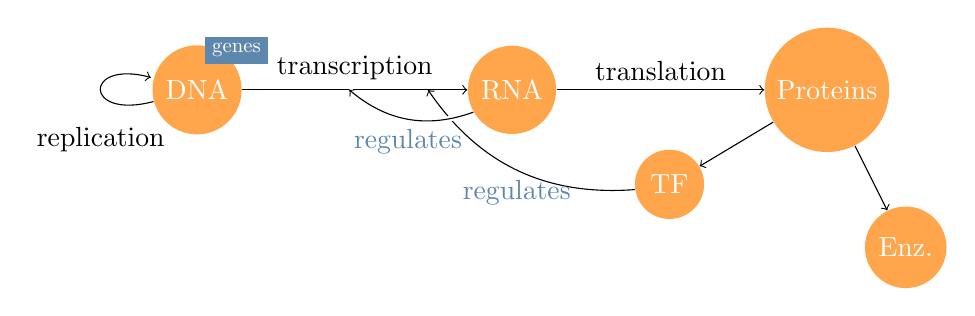
\begin{tikzpicture}
    \tikzstyle{every state}=[fill=orange!70!white,draw=none,text=white]
      
    \node[state] (dna) at (0,0) {DNA};
    \node[state] (rna) at (4,0) {RNA};
    \node[state] (proteins) at (8,0) {Proteins};
    \node[state] (tf) at (6,-1.2) {TF};
    \node[state] (enzyme) at (9,-2) {Enz.};
    \node[draw=none,text=white,fill=mblue, scale=0.75] (gene) at (0.5,0.5) {genes};
    
    \path
    (dna) edge [->] node[above] {transcription} (rna) 
    (rna) edge [->] node[above] {translation} (proteins) 
    (dna) edge [loop left,->] node[below=10pt] {replication} (dna) 
    (proteins) edge [->] node {} (tf) 
    (proteins) edge [->] node {} (enzyme) 
    (tf) edge [bend left, ->] node[below] {\textcolor{mblue}{regulates}} ($(rna.west) -(5mm,0)$)
    (rna) edge [-,line width=2pt,draw=white,bend left] ($(rna.west) -(15mm,0)$)
    (rna) edge [bend left, ->] node[below] {\textcolor{mblue}{regulates}} ($(rna.west) -(15mm,0)$);
  \end{tikzpicture}    
  \caption{Basic example of a multiattribute network in genomics:
    activity  of a  gene  can  be measured  at  the transcriptomic  and
    proteomic levels, and gene regulation affected accordingly}
\label{fig:central_dogma}
\end{figure}

\paragraph*{Why multiattribute networks?}  The need for
multiattribute networks is relevant in many application fields, but
seems particularly applicable in genomics.  Indeed, with the plurality
of emerging technologies and sequencing techniques, it is possible to
record many signals related to the same set of biological features at
various scales or locations of the cell.  Consider for instance the
simplifying -- still hopefully didactic -- central dogma of molecular
biology, sketched in Figure \ref{fig:central_dogma}: basically,
expression of a gene encoding for a protein can be measured either at
the transcriptome level, in terms of its quantity of mRNA, or at the
protein level, in terms of the concentration of the associated
protein.  Still, different technologies are used to measure either the
transcriptome or the proteome, typically, microarray or sequencing
technology for gene expression levels and cytometric or
immunofluorescence experiments for protein concentrations.  Although
these signals are very heterogeneous (different levels of noise, count
vs. continuous data, etc.), they do share commonality as they undergo
common biological processes.  We then put an edge in the network if it
is supported in both spaces (gene and protein spaces).  Our hope is
that molecular profiles combined on the same set of biological samples
can be \textit{synergistic}, in order to identify a ``consensus'' and
hopefully more robust network.

\paragraph*{multiattribute GGM.}   Let $\mathcal{P}=\{1,\dots,p\}$ be
a  set  of  variables  of  interest, each  of  them  having  some  $K$
attributes.    Consider  the   random   vector  $X   =  (X_1,   \dots,
X_p)^\intercal$  such  as  $X_i  =(X_{i1},\dots,X_{iK})^\intercal  \in
\mathbb{R}^K$ for $i\in\mathcal{P}$. The vector $X\in \mathbb{R}^{pK}$
describes the  $K$ recorded signals  for the $p$ features.   We assume
that $X$ is a multivariate centered  Gaussian vector, that is, $X \sim
\mathcal{N}(\mathbf{0}, \bSigma)$,  with covariance  and concentration
matrices defined block-wise
\[
\bSigma = \begin{bmatrix}
  \bSigma_{11} & & \bSigma_{1p} \\
  & \ddots & \\
  \bSigma_{p1} & & \bSigma_{pp} \\
\end{bmatrix}, \ \invcov = \begin{bmatrix}
  \invcov_{11} & & \invcov_{1p} \\
  & \ddots & \\
  \invcov_{p1} & & \invcov_{pp} \\
\end{bmatrix}, \quad \bSigma_{ij}, \invcov_{ij}\in \mathcal{M}_{K,K},
\ \forall (i,j)\in\mathcal{P}^2,
\]
where $\mathcal{M}_{a,b}$ is the set  of real-valued matrices with $a$
rows, $b$ columns.   Such a multiattribute framework  has been studied
in \cite{katenka2012inference} with a reconstruction method based upon
canonical  correlations in  order to  test dependencies  between pairs
$(i,j)$ at the attribute level  using covariance.  Here, we propose to
rely on partial  correlations in a multivariate  framework rather than
(canonical)  correlations   to  describe  relationships   between  the
features, and  thus extend  GGM to  a multiattribute  framework.  The
objective   is  to   define   a  ``canonical''   version  of   partial
correlations.      In    our     setting,    the     target    network
$\graph=(\mathcal{P},\mathcal{E})$  is  defined  as  the  multivariate
analog of the conditional graph for univariate GGM, that is
\begin{equation}
  \label{eq:multi_net}
  (i,j)  \in  \mathcal{E}  \Leftrightarrow \invcov_{ij}  \neq  \bzr_{KK},
  \quad \forall i\neq j.
\end{equation}
In words,  there is  no edge  between two variables  $i$ and  $j$ when
their attributes are all conditionally independent.

\paragraph*{A multivariate version of neighborhood selection.}  Our
idea for performing sparse multiattribute GGM inference is to define
a multivariate analog of the neighborhood selection approach
\cite{2006_AS_Meinshausen} (see Section \ref{sec:sparseGGM}, Equations
\eqref{eq:Lasso_MB} and \eqref{eq:MB_pseudo}). Indeed, it seems to be
the most natural and convenient setup toward multivariate
generalization.  Nevertheless, other sparse GGM inference method like
the graphical-Lasso \eqref{eq:MLE_l1} should have an equivalent
multiattribute version. A possibility is explored in
\cite{kolar2014graph} for instance.

To extend the neighborhood selection approach to a multiattribute
version, we look at the multivariate analog of equation
\eqref{eq:lincoef2invcov}: in a multivariate linear regression setup,
it is a matter of straightforward algebra to see that the conditional
distribution of $X_j\in\Rset^K$ on the other variables is
\begin{equation*}
  X_j \, |\,  X_{\backslash j}  = x \sim  \mathcal{N}(- \invcov_{jj}^{-1}\invcov_{j
    \backslash j} x , \invcov_{jj}^{-1})\enskip.
\end{equation*} 
Equivalently,     letting      $\displaystyle     \mathbf{B}_j^T     =
-\invcov_{jj}^{-1} \invcov_{j\backslash j}$, one has
\begin{equation*}
  X_j \, |\, X_{\backslash j} = \mathbf{B}_j^T X_{\backslash j} +
  \boldsymbol\varepsilon_j \quad \boldsymbol\varepsilon_j
  \sim \mathcal{N}(\mathbf{0},\invcov_{jj}^{-1}), \quad \boldsymbol\varepsilon_j \perp X,
\end{equation*}
where $\mathbf{B}_j\in\mathcal{M}_{(p-1)K,K}$ is defined block-wise
\begin{equation*}
  \mathbf{B}_j = \begin{bmatrix}
    \mathbf{B}_j^{(1)} \\ \hline
    \vdots \\ \hline
    \mathbf{B}_j^{(j-1)} \\ 
    \mathbf{B}_j^{(j+1)} \\ 
    \vdots \\ \hline
    \mathbf{B}_j^{(p)} \\ 
  \end{bmatrix} = - \begin{bmatrix}
    \invcov_{j1} \\ \hline
    \vdots \\ \hline
    \invcov_{j(j-1)} \\ 
    \invcov_{j(j+1)} \\ 
    \vdots \\ \hline
    \invcov_{j(p)} \\ 
  \end{bmatrix}^\top \times \invcov_{jj}^{-1},
\end{equation*}
and where each $\mathbf{B}_j^{(i)}$ is a $K\times K$ matrix which
links attributes of variables $(i,j)$.  We see that recovering the
support of $\bB_j$ block-wise is equivalent to reconstructing the
network defined in \eqref{eq:multi_net}.  Estimation of $\bB_j$ is
thus typically achieved through sparse methods.  To this end, we
consider an i.i.d.  sample $\{X^\ell\}_{\ell=1}^n$ of $X$ such that
each attribute is observed $n$ times for the $p$ variables, each $X^n$
being a $pK$-size row vector staked in a $\mathcal{M}_{n,pK}$ data
matrix $\mathbf{X}$ , so that $\bX_j \in \mathcal{M}_{n,K}$ is a
real-value, $n \times K$ block matrix containing the data related to
the $j$th variable:
\begin{multline*}
  \mathbf{X} = \begin{bmatrix}
    \mathbf{x}^1 \\ \hline
    \vdots \\\hline
    \mathbf{x}^n \\
  \end{bmatrix}
  = \begin{bmatrix}
    \mathbf{X}_1 & \dots & \mathbf{X}_p \\
  \end{bmatrix} 
  = \begin{bmatrix}
    X_{11}^1 & \dots & X_{1K}^1 & \vline & \dots & \vline & X_{p1}^1 & \dots & X_{pK}^1 \\ \hline
    \vdots & & \vdots & \vline & \dots & \vline & & & \\ \hline
    X_{11}^n & \dots & X_{1K}^n & \vline & \dots & \vline & X_{p1}^n & \dots & X_{pK}^n \\ 
  \end{bmatrix}.
\end{multline*}

Using  these notations,  a direct  generalization of  the neighborhood
selection is to  predict for each $j=1,\dots,p$ the  data block $\bX_j$
by regressing  on $\bX_{\backslash  j}$. In matrix  form, this  can be
written as the optimization problem
\begin{equation}
  \label{eq:multi_penalized}
  \arg  \min_{\bB_j  \in  \mathbb{R}}  J(\bB_j),  \qquad
  J(\bB_j) = \frac{1}{2n} \left\|
    \bX_j - \bX_{\backslash j}\bB_j\right\|_F^2 +
  \lambda \ \Omega(\bB_j),
\end{equation}
where $\|\bA\|_F = \sqrt{\sum_{i,j} \bA_{ij}^2}$ is the Frobenius norm
of  matrix   $\bA$  and  $\Omega$   is  a  penalty   which  constrains
$\mathbf{B}_j$ block-wise.

\paragraph{Choosing  a penalizer.}   Various choices  for $\Omega$  in
\eqref{eq:multi_penalized}   seem   relevant:    by   simply   setting
$\Omega_0(A) = \sum_{i,j} |A_{i,j}|$, we just encourage sparsity among
the $\mathbf{B}_i$  and thus do  not couple the attributes.   A clever
choice would be to activate a set of attributes all together: hence, the
group is defined  by all the $K$ attributes between  variables $i$ and $j$,
therefore the penalizer turns to a group-Lasso like penalty
\begin{equation}
  \label{eq:penalty_grp_variate}
  \Omega_1(\mathbf{B}_j) = \sum_{i \in \mathcal{P}\backslash j} \|\mathbf{B}_j^{(i)}\|_F,
\end{equation}
in  which  case  convex  analysis  and  subdifferential  calculus  (see
\cite{2006_CO_Boyd})  can be  used to  show that  a $\mathbf{B}_i$  is
optimal for Problem \eqref{eq:multi_penalized} iff
\begin{equation}
  \label{eq:optimality}
  \left\{\begin{array}{lrl}
      \forall i : \mathbf{B}_j^{(i)} \neq 0, & \left(\mathbf{S}_{ij} +
        \frac{\lambda}{\|\mathbf{B}_j^{(i)}\|_F           }          I
      \right)^{-1} \mathbf{S}_{ij} & = \mathbf{B}_j^{(i)} \\ 
      \forall i : \mathbf{B}_j^{(i)} = \bzr_{KK}, & 
      \| \mathbf{S}_{ij} \|_F & \leq \lambda \\
  \end{array}\right.,
\end{equation}
where  $\bS_{ij}\in\mathcal{M}_{KK}$ is  a  $K\times K$  block in  the
empirical covariance matrix $\bS_n  = n^{-1} \bX^\top\bX$, which shows
the  same block-wise  decomposition as  $\bSigma$ or  $\bTheta$.  This
paves  the way  for  an optimization  algorithm like  block-coordinate
descent which we implemented, although we omit details here. 



\section{Numerical  experiments}

\paragraph*{Simulation study.} We propose a simple simulation to
illustrate the interest of using multiattribute networks.  The
simulations are set up as follows:
\begin{enumerate}
\item  Draw  a random  undirected  network  with  $p$ nodes  from  the
  Erd\"os-Renyi model with adajacency matrix $\bA$;
\item  Expand the  associated adjacency  matrix to  multivariate space
  with
  $$\mathbf{M} = \mathbf{A}  \otimes \mathbb{S} + \mathbf{I}_{p\times K}$$
  where $\otimes$ is the Kronecker product. The $K\times K$ matrix
  $\mathbb{S}$ is used to consider different scenarios of agreement
  across the attributes of two genes. We consider three cases
  \begin{enumerate}
  \item $\mathbb{S} = \mathbf{I}_{K,K}$ the $K\times K$ identity
    matrix: same intra-attribute network and no inter-attribute
    interactions;
  \item $\mathbb{S} = \mathbf{I}_{K,K} - \mathbf{1}_{K,K}$, same
    inter-attribute interactions and no intra-attribute interactions;
  \item $\mathbb{S} = \mathbf{1}_{K,K}$ a matrix full of one: full
    agreement between  attributes.
  \end{enumerate}
\item Compute $\bTheta$ a positive definite approximation of
  $\mathbf{M}$ by replacing null and negative eigenvalues by a small constant;
\item Control the difficulty of  the problem with $\gamma>0$ such that
  $\bTheta= \bTheta+ \gamma I$;
\item Draw an i.i.d. $n$-size sample $\bX\in\Rset^{n\times pK}$ of
  $X \sim \mathcal{N} \left( 0,\invcov^{-1} \right) .$
\end{enumerate}

We choose small networks with $p=40$, with $40$ edges on average and
vary $n$ from $p/2$ to $2p$. We fix $\gamma$ to $0.1$ and consider
cases where the number of attributes is $K=2,3$ and $4$. We compare
our multiattribute approach of neighborhood selection to two
baselines:
\begin{enumerate}
\item the standard neighborhood selection procedure applied on the
  data related to each attribute separately: to do so, we separate
  $\bX$ in $K$ data sets $\bX^{(1)}, \dots \bX^{(K)}$ all with size
  $\Rset^{n\times p}$ and reconstruct one network per attribute. We refer to
  this method as the \textit{separate} variant. It is very specific to
  each attribute and do not share at all the information across the
  attributes.  
\item the standard neighborhood selection approach applied on a merge
  data set, obtained by stacking the data sets
  $\bX^{(1)}, \dots \bX^{(K)}$ of each attribute into a single
  $\tilde\bX$ data set in $\Rset^{nK \times p}$. We refer to this
  method as the \textit{merge} variant. This method is the exact
  opposite of the \textit{separate} variant.
\end{enumerate}
We assess the performances of each method in reconstructing the
original adjacency matrix $\bA$ with the area under ROC curve
(AUC). For the \textit{separate} variant, the retained AUC is the AUC
averaged over all attributes. We replicate the experiment 100 times.

On Figure \ref{fig:simu_multi}, it is clear that aggregation (either
by merging data sets or with multiattribute network inference)
improves upon a single-attribute approach. Even when there is no
inter-attributes interactions, (which is barely meaningful towards
application to regulatory networks), in which case it is a very good
idea to merge the problems together to increase the sample size, our
multiattribute approach remains quite competitive and robust. In all
other cases, it outperforms the competing approaches.
\begin{figure}[htbp!]
  \centering
  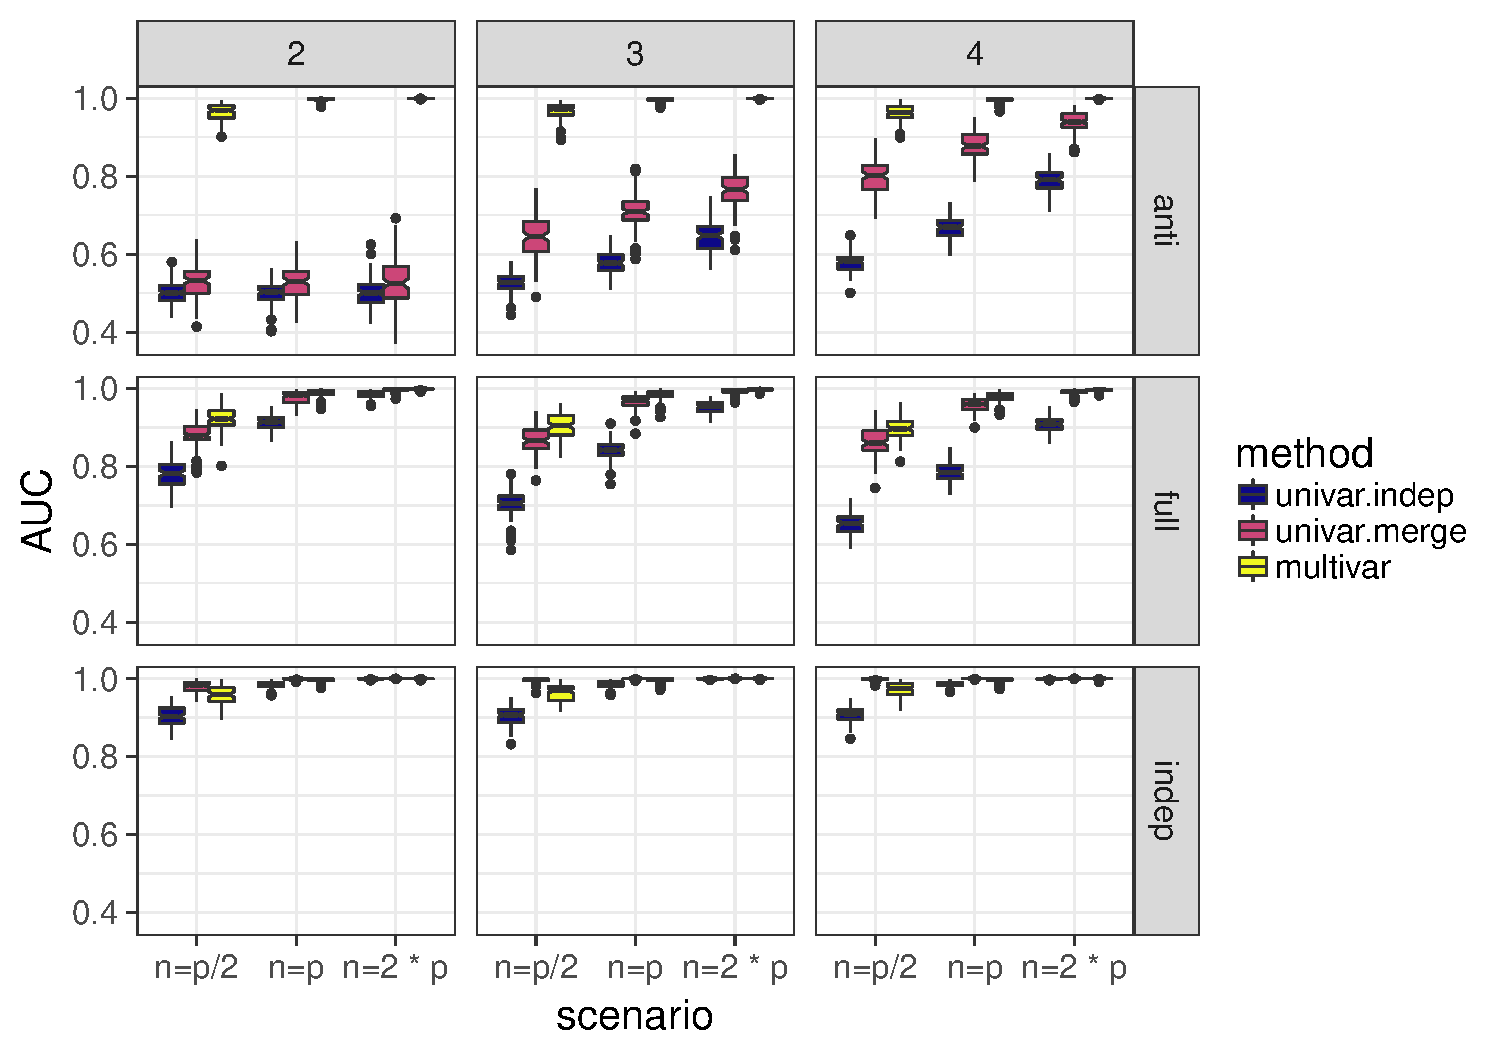
\includegraphics[width=\textwidth]{figures/res_simu_new}
  \caption{Simple simulation study for the multiattribute network
    inference problem: the multiattribute procedure improves over the
    univariate procedures in every situation when networks are close
    for each attribute.}
  \label{fig:simu_multi}
\end{figure}


\paragraph*{Illustration: Gene/Protein regulatory network inference.}

As an illustration, we applied our sparse multiattribute GGM approach
to reconstruct networks on two large breast cancer data sets from the
National Cancer Institute\footnote{\url{https://www.cancer.gov/}} and
the Rational Therapy for Breast Cancer
consortium\footnote{\url{http://www.ratherproject.com/}}, respectively
referred to as NCI-60 and RATHER hereafter. These data sets contain
both proteomic and transcriptomic profiles, respectively measured with
reverse-phase protein arrays (RPPA) and RNA affymetrix array. We infer
the multiattribute network between the subset of molecular entities
which is common to the proteins measured by RPPA and the genes
measured by RNA array, that we call the \textit{consensus set}: in the
NCI-60 cancer line data set \citep{pfister2009topoisomerase}, a
consensus set composed of $p=91$ protein and corresponding gene
profiles is retained, for the $n=60$ samples. The RATHER data set
\citep{michaut2016integration} contains proteomic and transcriptonic
data from $n=100$ patients for a consensus set of $p=117$
entities\footnote{The data can be downloaded from
  \url{https://www.ncbi.nlm.nih.gov/geo/query/acc.cgi?acc=GSE66647}.}.

We infer a sparse GGM for each attribute (gene expression and protein
profile), separately to start with, and then get its multiattribute
version.  We do this on a large grid of the tuning parameter and thus
have three families of networks indexed by their number of edges.

Figure \ref{fig:jaccard} demonstrates that our sparse multiattribute
method captures the characteristics of both univariate networks, as
the Jaccard similarity index is high between each uni-attribute
network and the multiattribute network, while it remains low when
comparing uni-attribute networks together.
\begin{figure}[htbp!]
  \centering
  \begin{tabular}{@{}cc@{}}
   RATHER & NCI-60 \\
    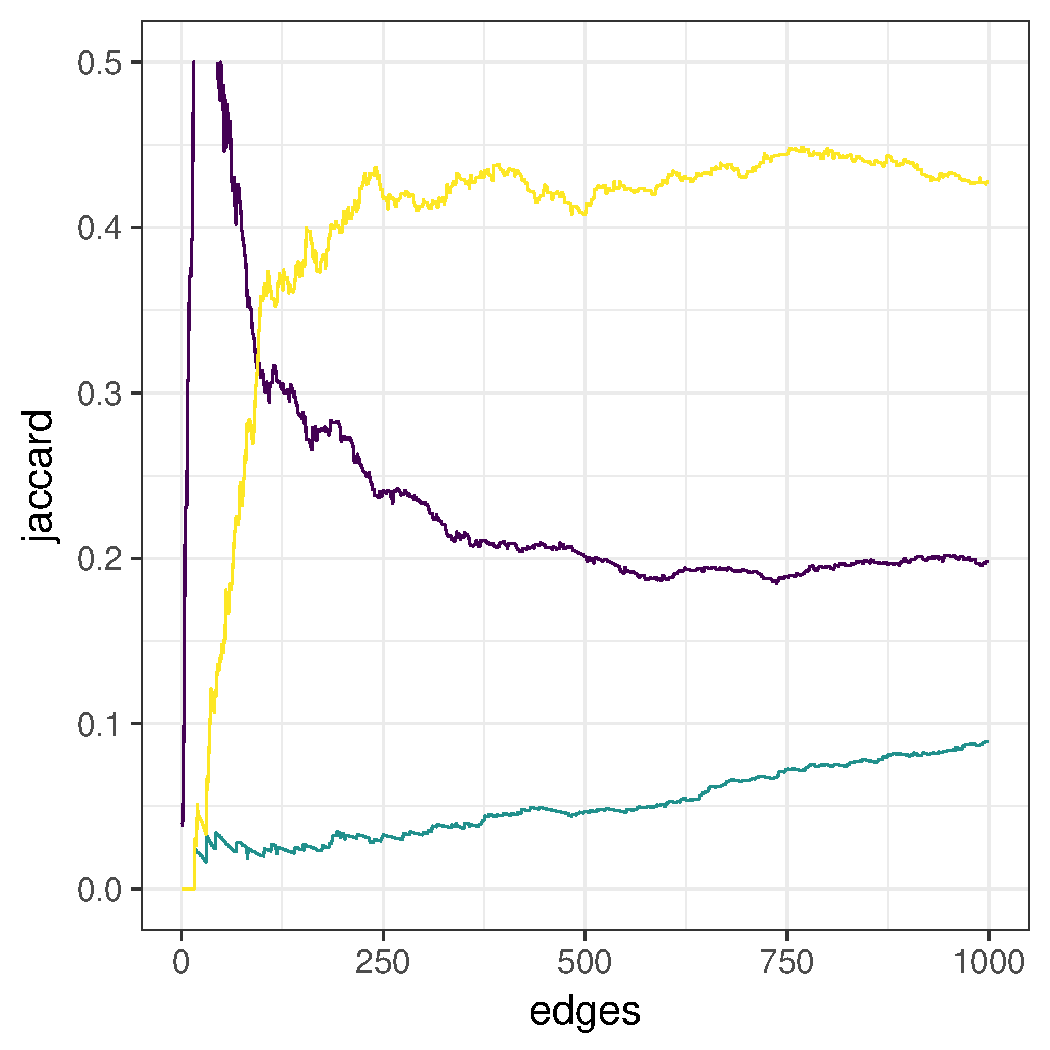
\includegraphics[width=.35\textwidth]{figures/jaccard_RATHER}
  & 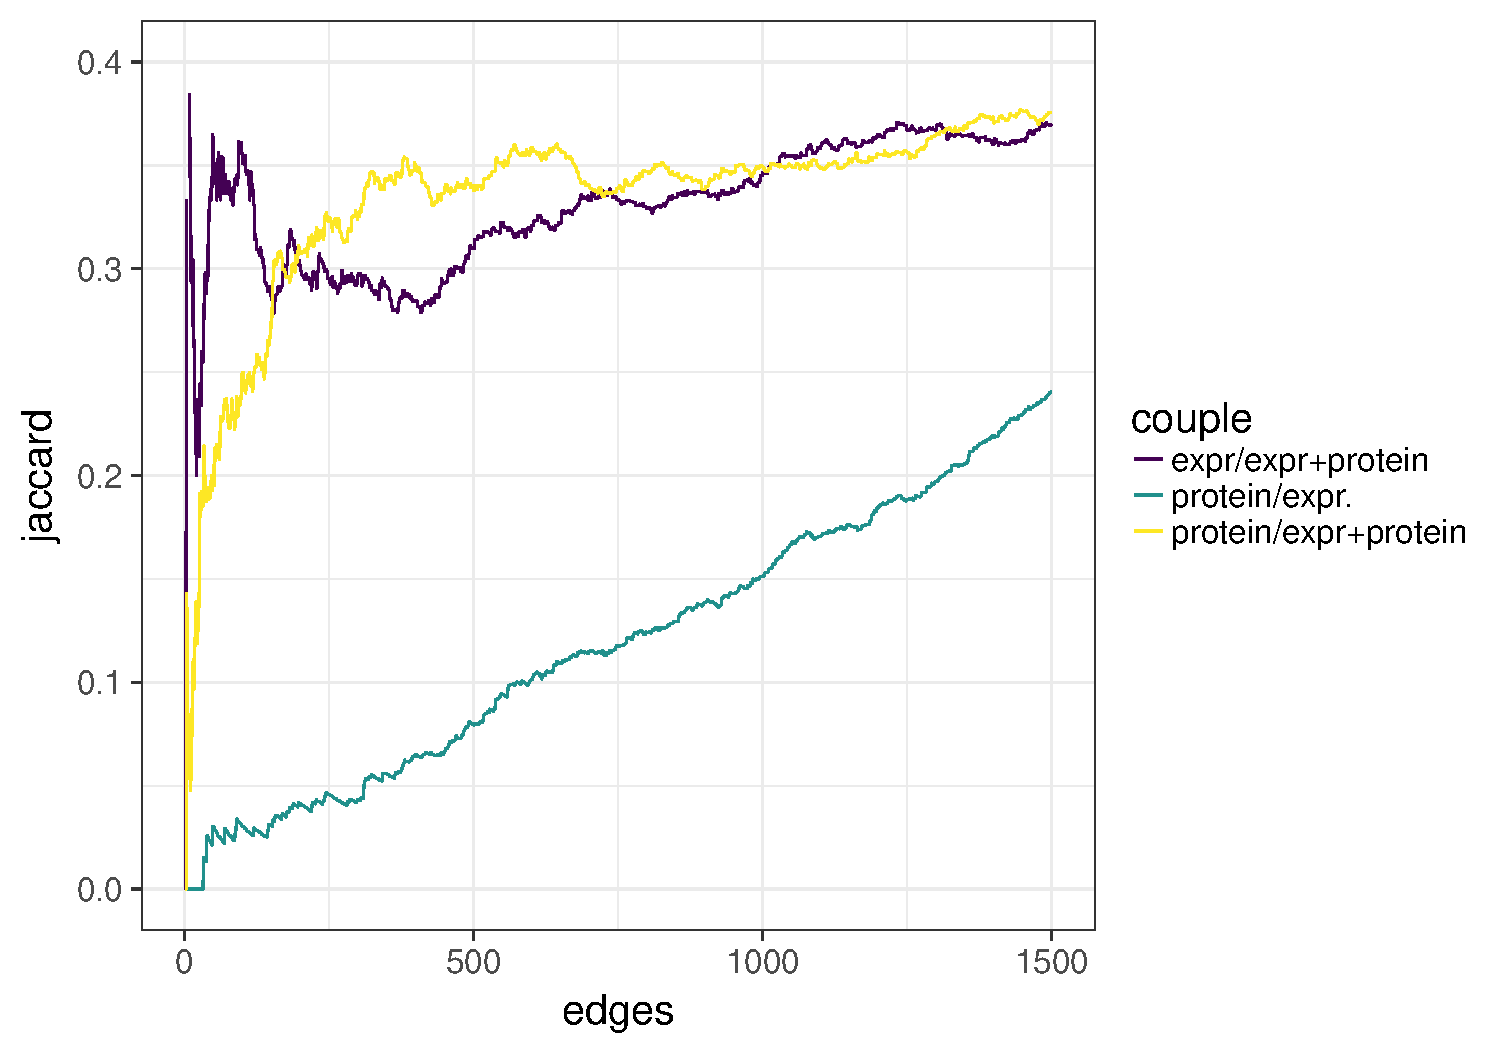
\includegraphics[width=.5\textwidth]{figures/jaccard_NCI60}
  \end{tabular}
  \caption{Jaccard's similarity index
    $J(A,B) = \frac{\left|A\cap B\right|}{\left|A\cup B\right|}$
    between uni-attribute and multiattribute networks, for RATHER and
    NCI60 data set: multiattribute networks share a high Jaccard
    index with both uni-attribute networks.}
  \label{fig:jaccard}
\end{figure}

Figure \ref{fig:networks} shows the finally retained networks, where
the number of edges is controlled by the tuning parameter $\lambda$
chosen by 10-fold cross-validation. It is clear that some motifs only
present in each uni-attribute networks are caught in their
multiattribute counterparts. This tends to prove that the
multiattribute version proposes a consensus version of the
interactions at hand in the cell, and one which is hopefully more
robust to noise.
\begin{figure}[htbp!]
  \centering
  \begin{tabular}{@{}lccc@{}}
    & proteomic network  & genomic network  & multiattribute network \\
    \rotatebox{90}{\hspace{1.2cm}NCI60} 
    & 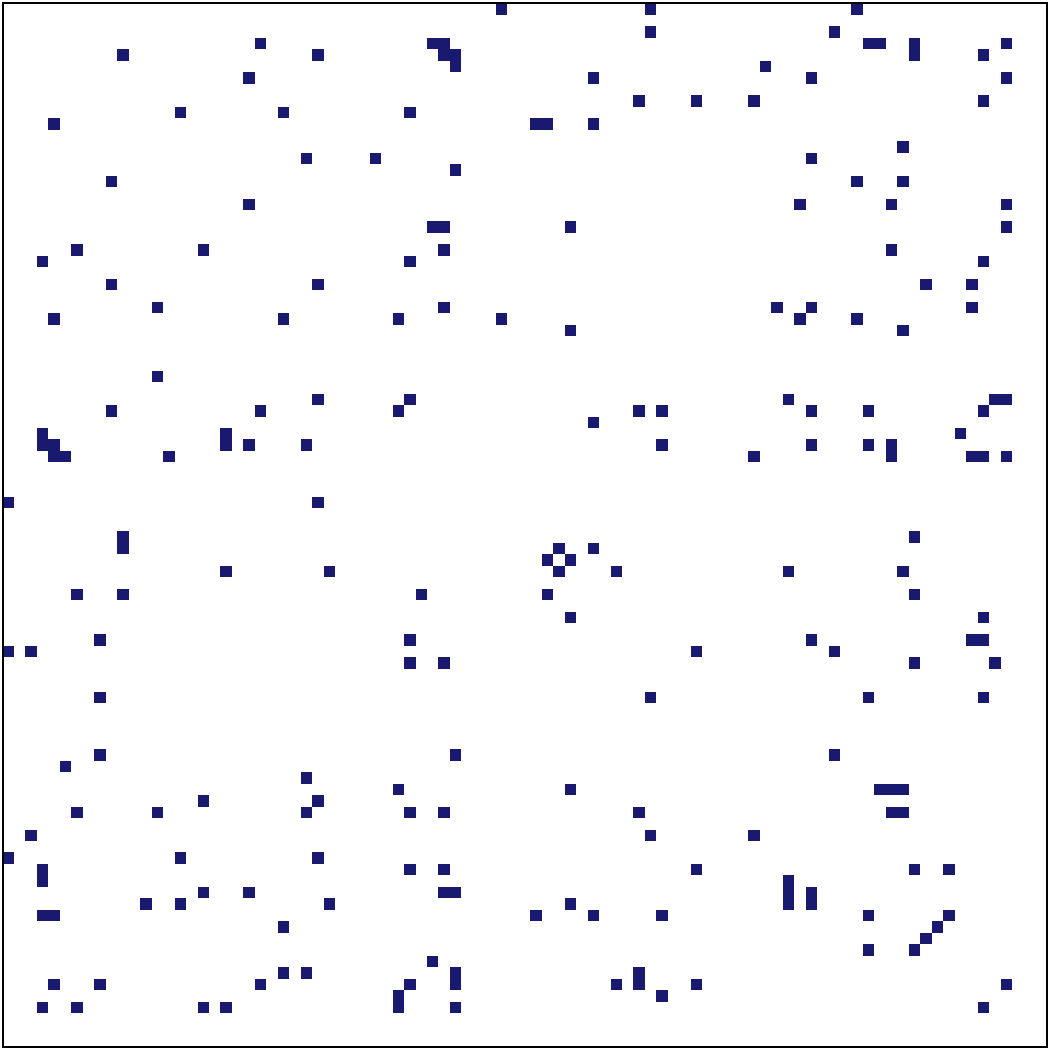
\includegraphics[width=.3\textwidth]{figures/protNet_NCI60}
    & 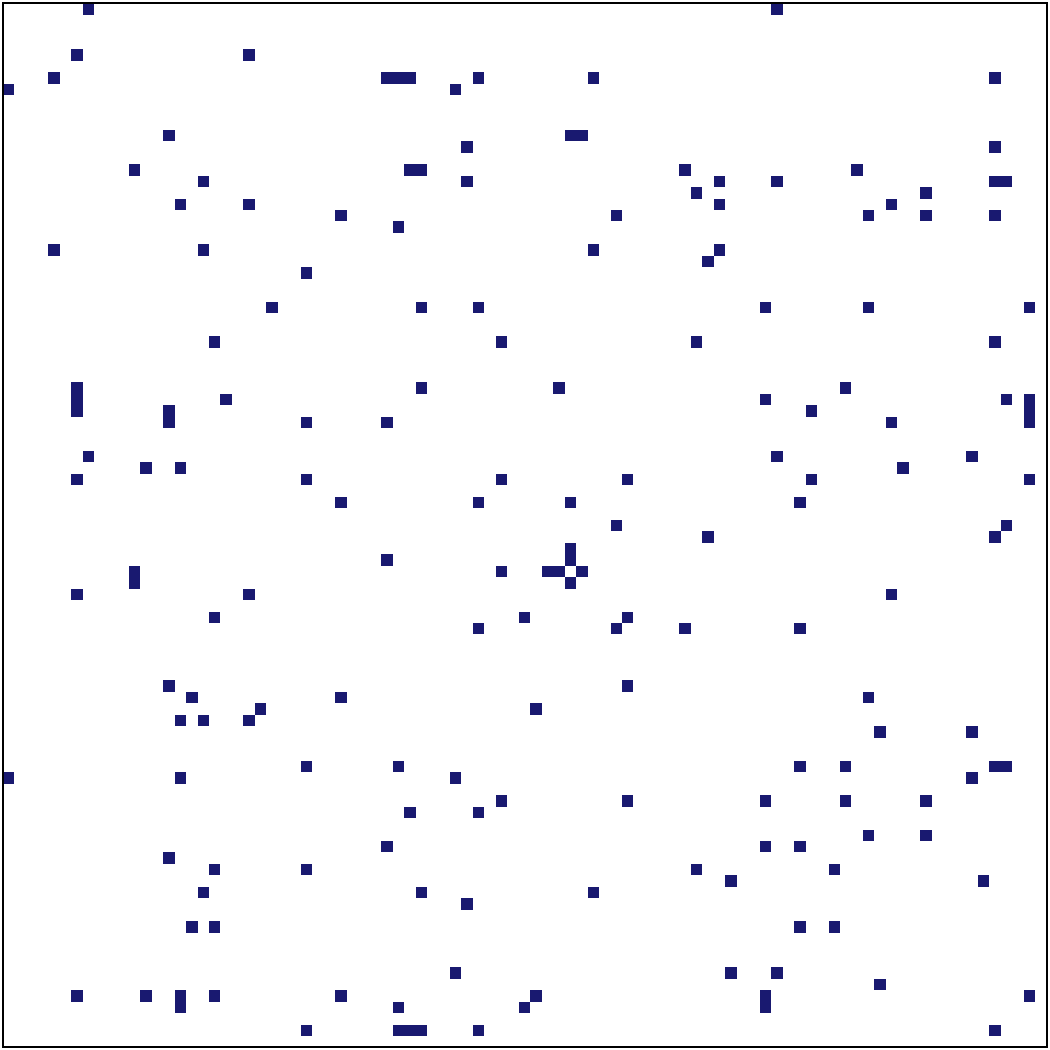
\includegraphics[width=.3\textwidth]{figures/exprNet_NCI60}
    & 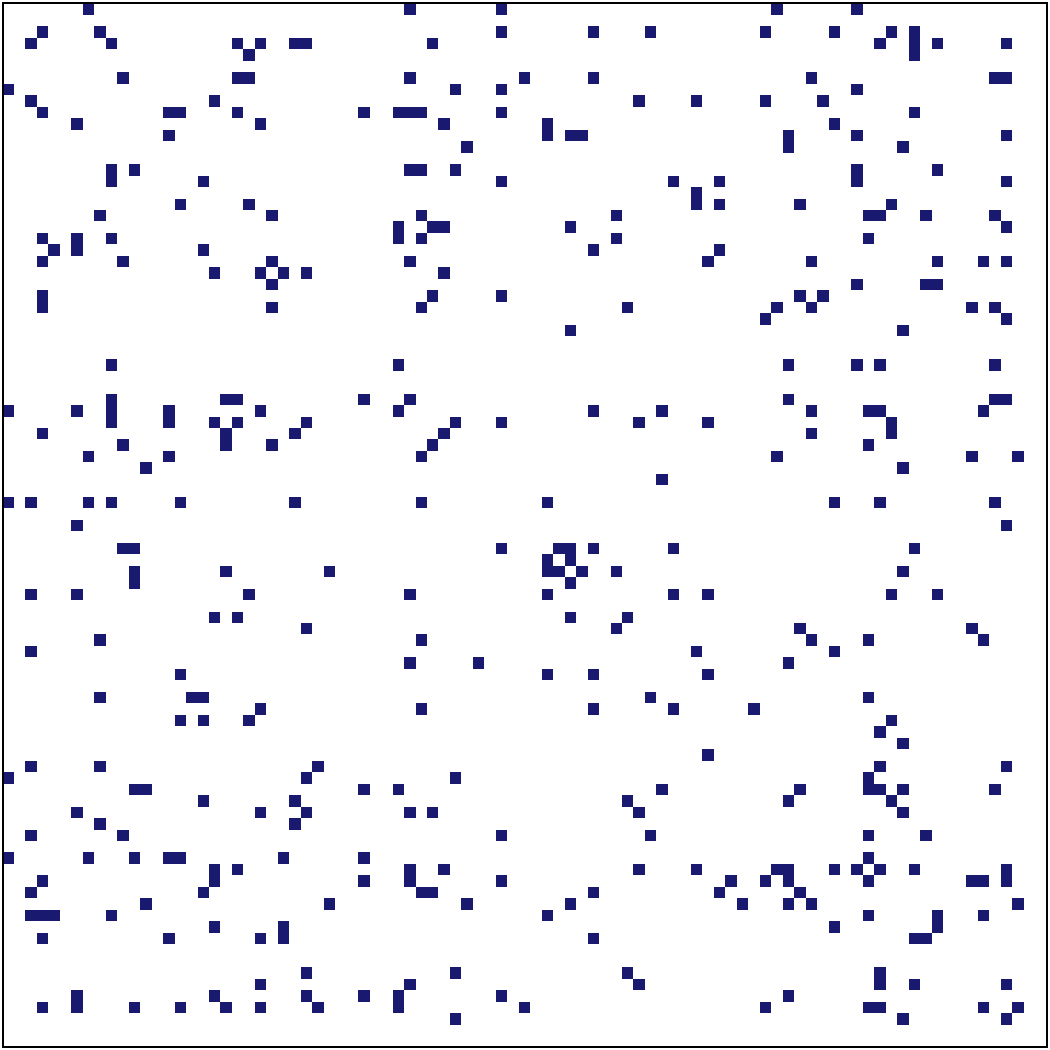
\includegraphics[width=.3\textwidth]{figures/bivarNet_NCI60} \\
    \rotatebox{90}{\hspace{1.2cm}RATHER} 
    & 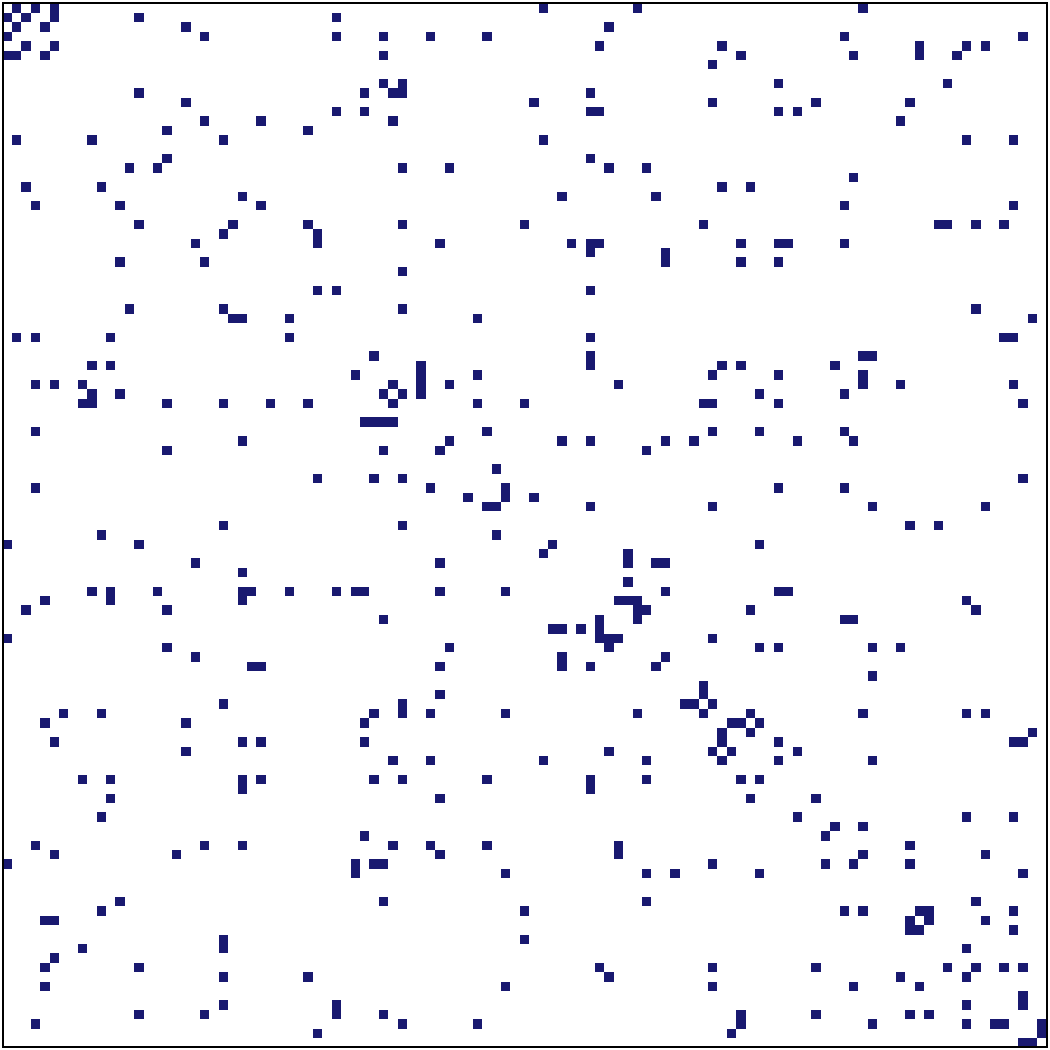
\includegraphics[width=.3\textwidth]{figures/protNet_RATHER}
    & 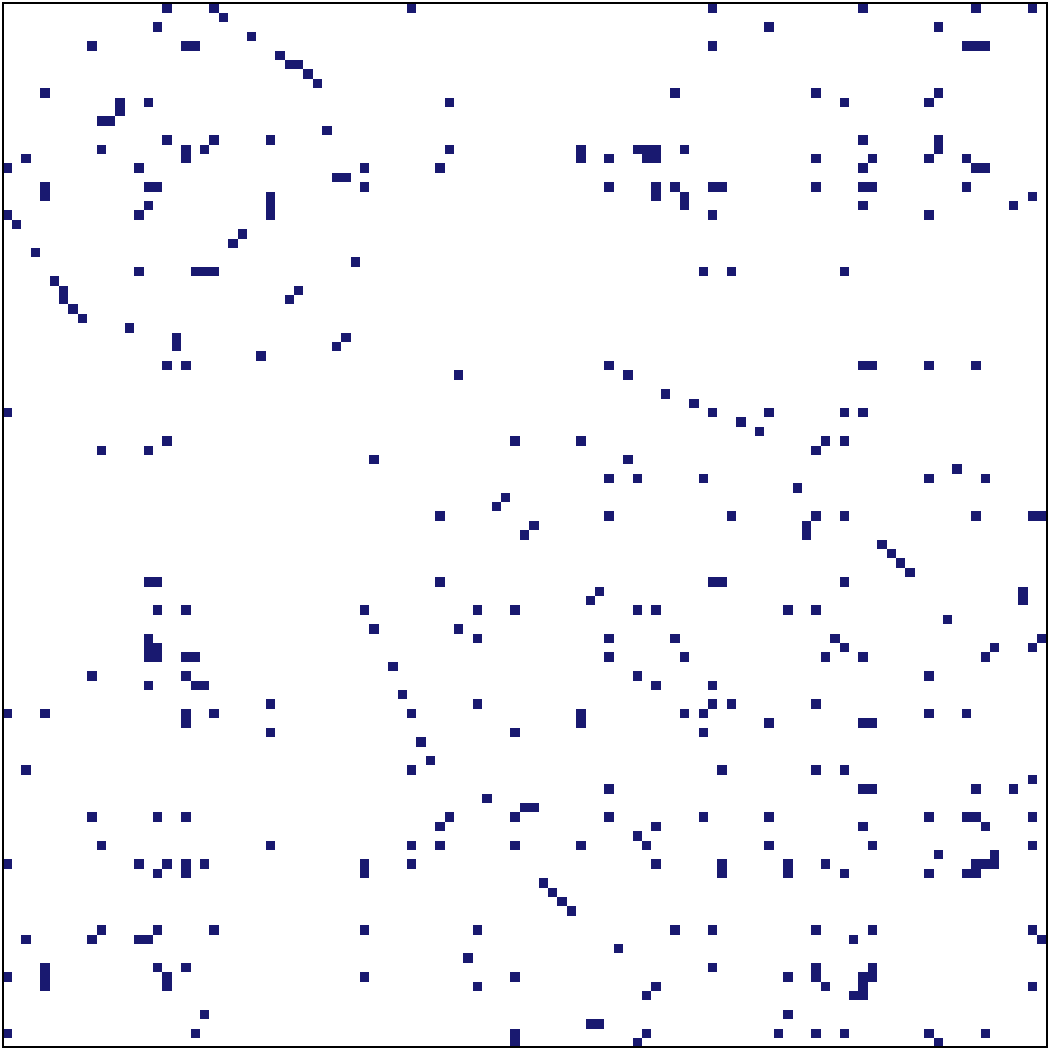
\includegraphics[width=.3\textwidth]{figures/exprNet_RATHER}
    & 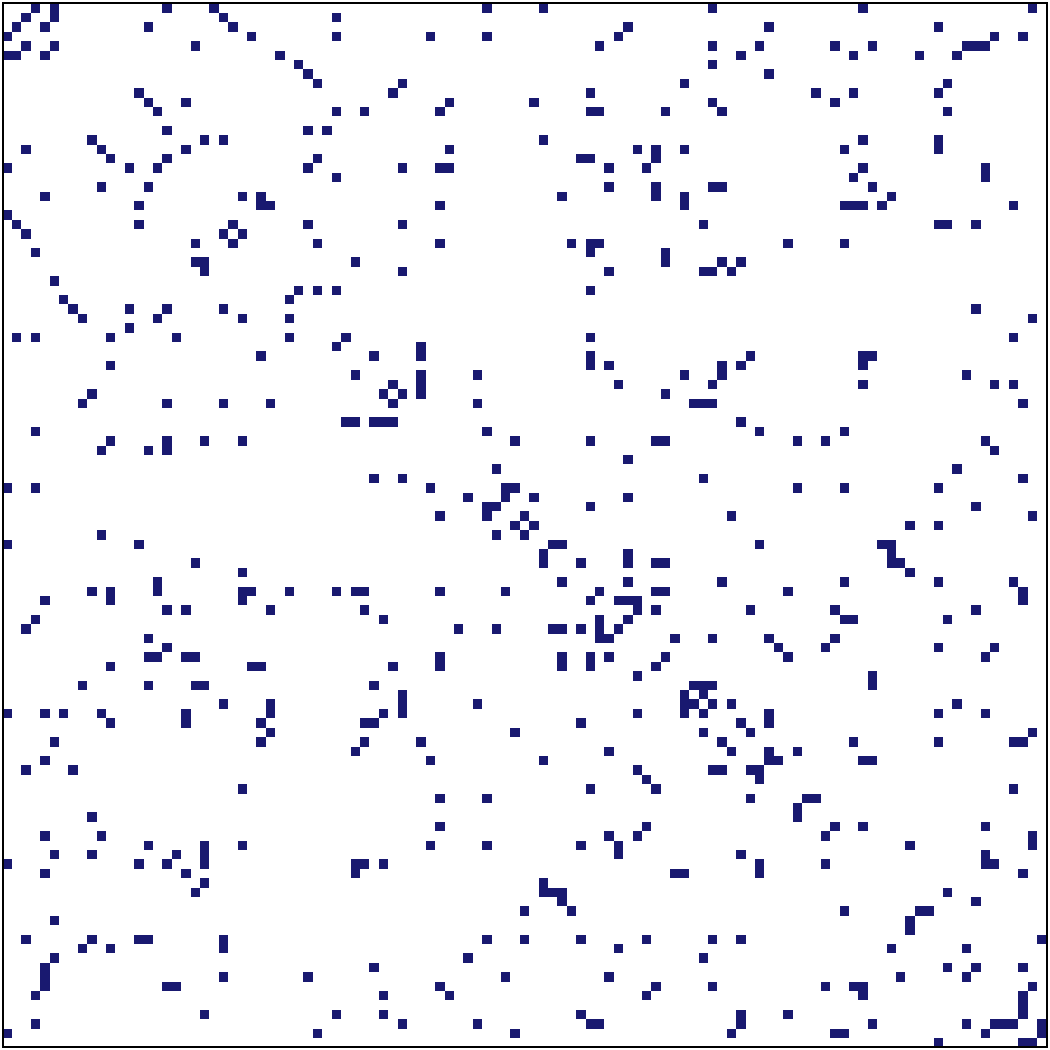
\includegraphics[width=.3\textwidth]{figures/bivarNet_RATHER} \\
  \end{tabular}
  \caption{Uni-attribute and multiattribute networks inferred on both
    NCI60 and RATHER dataset. The number of neighbors of each entity
    is chosen by cross-validation. Multiattribute networks catch motif
    found in the uniattribute counterparts.}
  \label{fig:networks}
\end{figure}





\bibliographystyle{spbasic}
\bibliography{biblio}

\end{document}

